
O Mastermind é um jogo de tabuleiro jogado entre 2 jogadores, em que
um deles cria um código secreto e o outro tenta-o descobrir num
determinado número de tentativas. Um exemplo de um tabuleiro, neste
caso num jogo de computador, pode ser visto na figura
\ref{fig:tabuleiro_mastermind}.

\begin{figure}[h!]
  \centering
    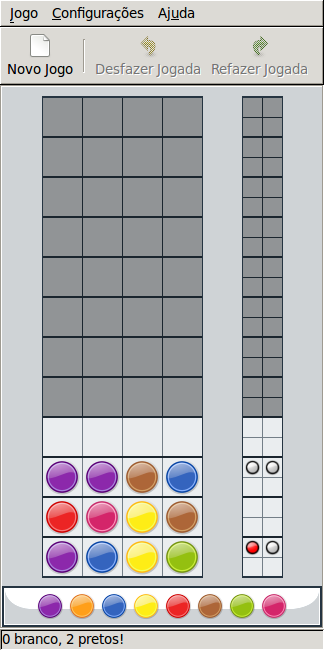
\includegraphics[scale=0.30]{gnome-mastermind.png}    
  \caption{Software que permite jogar o jogo Mastermind. Na situação
    mostrada o \emph{codebreaker} já efetuou 3 tentativas para adivinhar o código.}
  \label{fig:tabuleiro_mastermind}
\end{figure}



Inicialmente, o tabuleiro onde se vai efetuar o jogo encontra-se
limpo. Nesta altura, um dos jogadores, designado por \emph{codemaker}, cria,
utilizando as 6 cores disponíveis, um código de 4 cores. Este código
pode conter cores repetidas. Por exemplo, Azul, Azul, Azul, Azul é um
código válido.

Este código fica escondido, através de uma proteção existente no
tabuleiro, do outro jogador, designado por \emph{codebreaker}.

Após a criação do código por parte do \emph{codemaker}, o \emph{codebreaker} têm 12
tentativas para o tentar descobrir.

Cada tentativa processa-se da seguinte forma:
%
\begin{enumerate}
\item O \emph{codebreaker} escolhe um combinação de 4 cores que pensa ser a
  que o \emph{codemaker} criou;
\item O \emph{codemaker} observa a combinação escolhida pelo \emph{codebreaker} e
  compara-a com a que escolheu antes de começar o jogo;
\item Por cada cor que seja igual e esteja no mesmo sítio que uma cor
  do código original, o \emph{codemaker} coloca uma peça preta ao lado do
  código criado pelo \emph{codemaker};
\item Por cada cor que seja igual, mas esteja num sítio diferente que
  uma cor do código original, o \emph{codemaker} coloca uma peça branca ao
  lado do código criado pelo \emph{codemaker};
\end{enumerate}

Isto repete-se até que uma das seguintes situações ocorra:
%
\begin{enumerate}
\item O \emph{codemaker} coloca 4 peças pretas ao lado de uma tentativa feita
  pelo \emph{codebreaker}, indicando a este que o seu código está correto;
\item O \emph{codebreaker} não consegue descobrir o código criado pelo
  \emph{codemaker} no número de tentativas disponíveis.
\end{enumerate}

Se alguma destas situações ocorrer, então aquele jogo termina.

São atribuídos pontos ao \emph{codemaker} da seguinte forma:
%
\begin{itemize}
\item Se o \emph{codebreaker} descobriu o código, então o \emph{codemaker} ganha um
  número de pontos igual ao número de tentativas feitas pelo \emph{codebreaker};
\item Se o \emph{codebreaker} não descobriu o código, então o \emph{codemaker} ganha
  um número de pontos igual ao número de tentativas feitas mais 1.
\end{itemize}

Após este jogo terminar é realizado um outro jogo em que os papéis dos
jogadores estão invertidos, ou seja, o jogador que fez de \emph{codemaker}
passa a ser o \emph{codebreaker} e assim sucessivamente.

É então jogado um novo jogo como foi descrito anteriormente.

No final desse jogo, a partida termina e ganha quem tiver tido o maior
número de pontos, ou seja, ganha quem tiver feito o código mais
difícil de descobrir.


